\documentclass[border=5pt]{standalone}
\usepackage{amsmath}
\usepackage{tikz}
\usetikzlibrary{arrows.meta,positioning,shapes.geometric,fit}
\usepackage{times}

\begin{document}
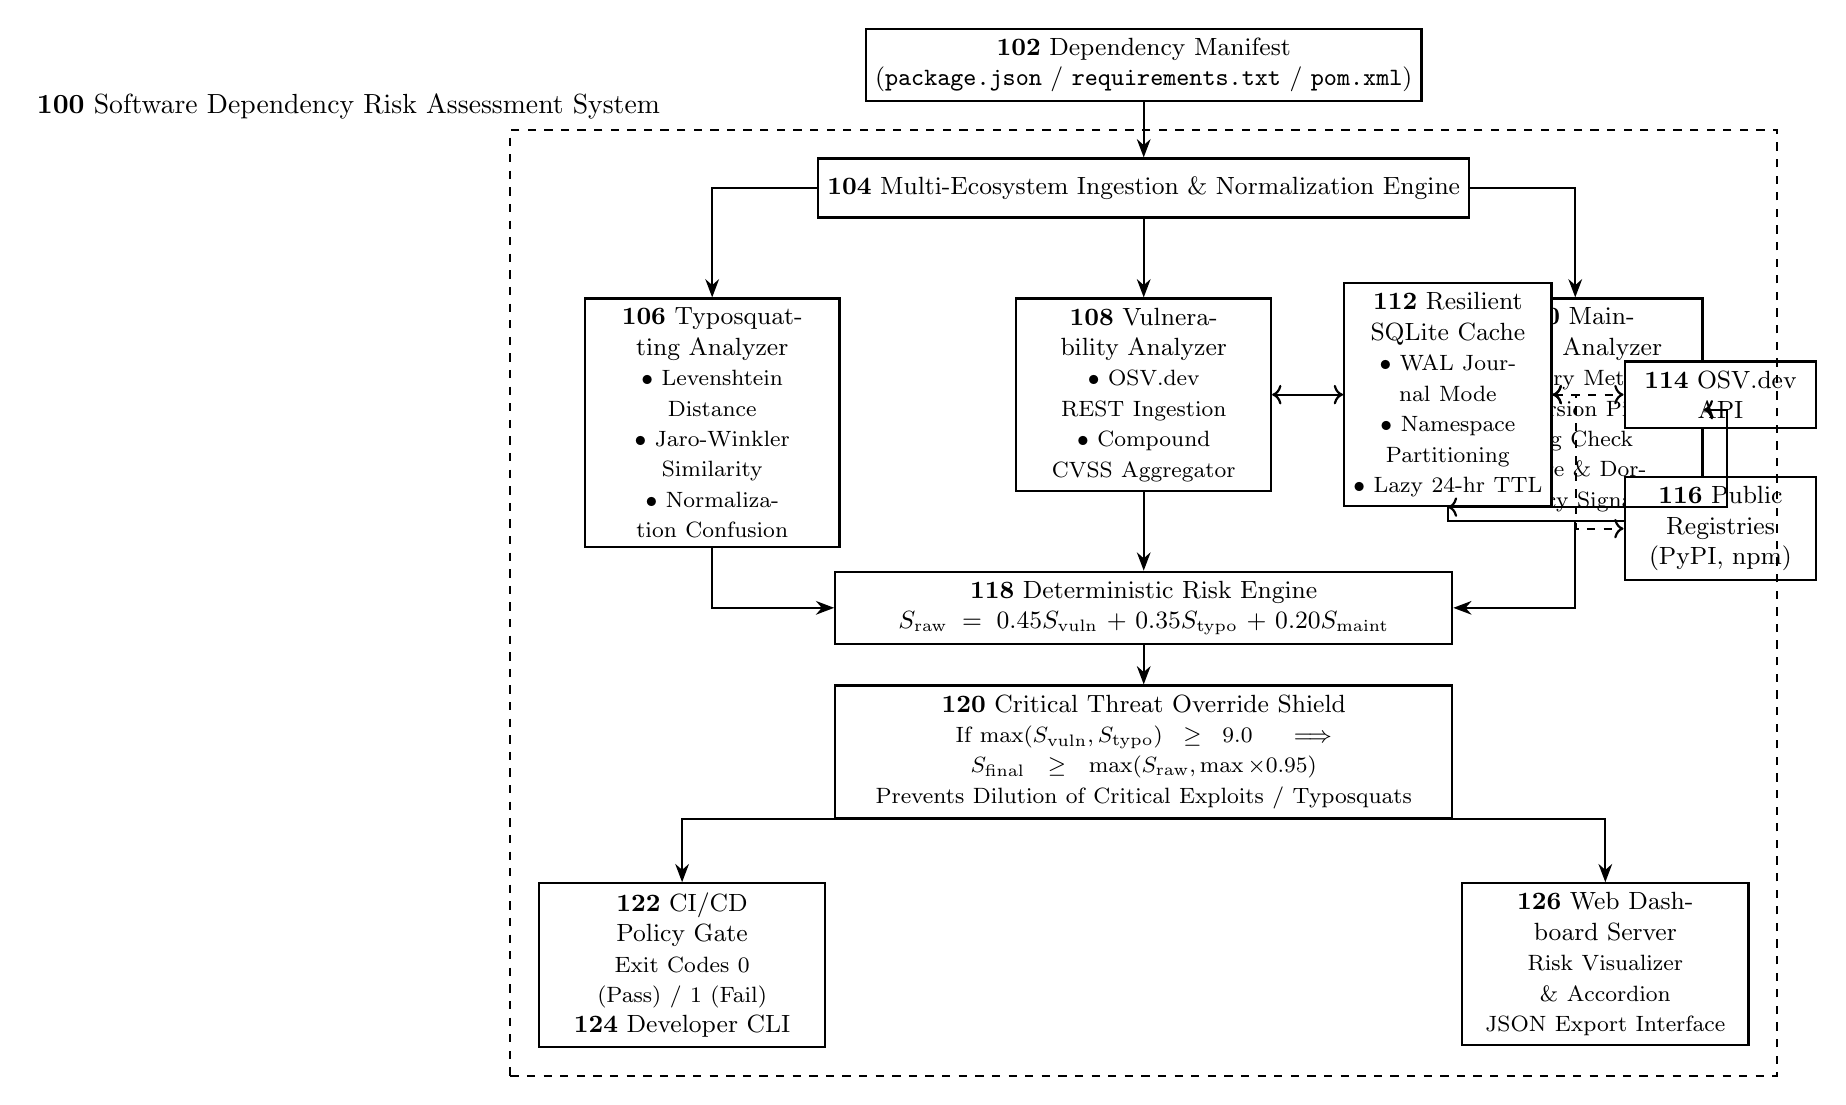
\begin{tikzpicture}[
    node distance=1.0cm and 0.8cm,
    box/.style={rectangle, draw=black, thick, fill=white, minimum height=0.75cm, align=center, font=\small},
    group/.style={rectangle, draw=black, dashed, thick, inner sep=0.35cm, font=\small},
    arrow/.style={-{Stealth[scale=1.0]}, thick, draw=black},
    num/.style={font=\bfseries\small}
]

% Boundary of the system
\node[box] (manifest) {\textbf{102} Dependency Manifest\\(\texttt{package.json} / \texttt{requirements.txt} / \texttt{pom.xml})};
\node[box, below=0.7cm of manifest] (parser) {\textbf{104} Multi-Ecosystem Ingestion \& Normalization Engine};
\draw[arrow] (manifest) -- (parser);

% Analyzers
\node[box, below left=1.0cm and -0.3cm of parser, text width=3.0cm] (typo) {
    \textbf{106} Typosquatting Analyzer\\
    {\footnotesize $\bullet$ Levenshtein Distance}\\
    {\footnotesize $\bullet$ Jaro-Winkler Similarity}\\
    {\footnotesize $\bullet$ Normalization Confusion}
};

\node[box, below=1.0cm of parser, text width=3.0cm] (vuln) {
    \textbf{108} Vulnerability Analyzer\\
    {\footnotesize $\bullet$ OSV.dev REST Ingestion}\\
    {\footnotesize $\bullet$ Compound CVSS Aggregator}
};

\node[box, below right=1.0cm and -0.3cm of parser, text width=3.0cm] (maint) {
    \textbf{110} Maintainer Analyzer\\
    {\footnotesize $\bullet$ Registry Metadata}\\
    {\footnotesize $\bullet$ Version Pinning Check}\\
    {\footnotesize $\bullet$ Age \& Dormancy Signals}
};

\draw[arrow] (parser) -| (typo.north);
\draw[arrow] (parser) -- (vuln.north);
\draw[arrow] (parser) -| (maint.north);

% Caching Store and External Services
\node[box, right=0.9cm of vuln, text width=2.4cm] (cache) {
    \textbf{112} Resilient SQLite Cache\\
    {\footnotesize $\bullet$ WAL Journal Mode}\\
    {\footnotesize $\bullet$ Namespace Partitioning}\\
    {\footnotesize $\bullet$ Lazy 24-hr TTL}
};
\node[box, right=0.9cm of cache, text width=2.2cm] (osv) {\textbf{114} OSV.dev API};
\node[box, below=0.6cm of osv, text width=2.2cm] (registry) {\textbf{116} Public Registries\\(PyPI, npm)};

\draw[<->, thick] (vuln) -- (cache);
\draw[<->, thick] (maint.east) -- ++(0.3,0) |- (cache.south);
\draw[<->, dashed, thick] (cache) -- (osv);
\draw[<->, dashed, thick] (cache.east) -- ++(0.3,0) |- (registry.west);

% Risk Engine
\node[box, below=1.0cm of vuln, text width=7.6cm] (engine) {
    \textbf{118} Deterministic Risk Engine\\
    $S_{\text{raw}} = 0.45 S_{\text{vuln}} + 0.35 S_{\text{typo}} + 0.20 S_{\text{maint}}$
};

\node[box, below=0.5cm of engine, text width=7.6cm] (override) {
    \textbf{120} Critical Threat Override Shield\\
    {\footnotesize If $\max(S_{\text{vuln}}, S_{\text{typo}}) \ge 9.0 \implies S_{\text{final}} \ge \max(S_{\text{raw}}, \max \times 0.95)$}\\
    {\footnotesize Prevents Dilution of Critical Exploits / Typosquats}
};

\draw[arrow] (typo.south) |- (engine.west);
\draw[arrow] (vuln.south) -- (engine.north);
\draw[arrow] (maint.south) |- (engine.east);
\draw[arrow] (engine) -- (override);

% Output Gateways
\node[box, below left=0.8cm and 0.1cm of override, text width=3.4cm] (cli) {
    \textbf{122} CI/CD Policy Gate\\
    {\footnotesize Exit Codes 0 (Pass) / 1 (Fail)}\\
    \textbf{124} Developer CLI
};

\node[box, below right=0.8cm and 0.1cm of override, text width=3.4cm] (dash) {
    \textbf{126} Web Dashboard Server\\
    {\footnotesize Risk Visualizer \& Accordion}\\
    {\footnotesize JSON Export Interface}
};

\draw[arrow] (override.south) -| (cli.north);
\draw[arrow] (override.south) -| (dash.north);

% Overall System Box
\node[group, fit=(parser) (typo) (vuln) (maint) (cache) (engine) (override) (cli) (dash), label=above left:{\textbf{100} Software Dependency Risk Assessment System}] (sys) {};

\end{tikzpicture}
\end{document}
